\section{Stand der Technik}

Für die Bezahlungsmethoden werden hier zwei verschiedene Arten von Zahlungsverfahren analysiert und deren
Vorteile in Bezug auf Sicherheit und Härtungsmaßnahmen dargestellt: drahtlose Zahlung und Kartenzahlung.

\subsection{Drahtlose Verbindungen und Sicherheit bei Bezahlungen}

Viele digitale Zahlungen finden über WLAN statt, was ein großes Risiko darstellen kann \cite{refip:NYRS}, 
da WLAN-Verbindungen nicht so sicher sind wie Kabelverbindungen. Maßnahmen zu entwickeln, die sich an 
verschiedenen Systeme anpassen, kosten Zeit und Investitionen von Banken und Sicherheitsfirmen. 
Für jeden möglichen Angriffe sollte präventiv etwas getan werden, sodass die Integrität 
\footnote{Es ist Subjekten nicht möglich, die zu schützenden Daten unatorisiert und unbemerkt zu manipulieren \cite{refbook:SWIS}.}
des Kunden geschützt bleibt. Die folgenden Schwachstellen bei digitaler Zahlung wurden von \cite{refip:NYRS}
zusammengefasst:

\begin{itemize}
    \item Erstellung von Dateien in dem Opfersystem mit umfangreichen Privilegien
    \item unzureichende Sicherheit bei der Validierung von Zertifikaten
    \item Quellcode ist öffentlich zugänglich, sodass das Opfersystem von Reverse
    Engineering\footnote{Reverse Engineering ist das Prozess von Identifzierung der Bestandteilen 
    eines Systems(Hardware bzw. Software) und von Wiederherstellung dieses Systems in einer anderen Format
    \cite{refart:CHRE}. In der Sicherheitsbereich wird Reverser Engineering verwendent, um Schwachstellen 
    von Hardware bzw. von Software zu entedecken, sodass diese ausgenutzt werden können \cite{refip:CMBM}.}: 
    betroffen sein kann
    \item Unsicherer Umgang mit Cookies-Einstellungen\footnote{Cookies sind Textdateien, die verwendet werden, um Nutzer und
    dessen Einstellungen im Netz zu identifizieren. Verschiedene Angriffe oder Manipulationen können stattfinden,
    wenn die Sicherheit bei der Erstellung von Cookies nicht berücksichtig ist \cite{refart:HSSC}.}.
\end{itemize}



\cite{refip:NYRS} schlägt einige Sicherheitsmechanismen vor, die die oben gennanten Schwachstellen bei 
kabelosen Verbindungen reduzieren können. Unter denen werden folgende hervorgehoben: 


\begin{itemize}
    \item Nutzung von modernen kryptographischen Standards für die Validierung von Zertifikaten
    \item Erstellung von Loggdateien, sodass jede Anormalität schnell bemerkt werden kann
    \item Zwei-Faktor-Authentifizierung
    \item digitale und zufällig geordnete Tastatur
    \item Schwierigkeitsgrad bei der Erstellung von Passwörtern
    \item besserer Umgang mit der Verwaltung von Cookies
    \item Registrierung von Geräten
    \item künstliche Intelligenz (KI) für die Detektion von abweichenden Verhalten
    \item ständige Kontrolle gegen Social Engineering \footnote{Beim Social-Engineering nutzt der Täter den ``Faktor Mensch'' als vermeintlich 
    schwächstes Glied der Sicherheitskette aus, um seine kriminelle Absicht zu verwirklichen.\cite{booklet:BSSE}}.
\end{itemize}


\textbf{Was können wir noch hinzufügen??? Lieber nichts!!!!}

Kredit- und EC-Karten sollen auch als Zahlungsmittel bei unserem Click-and-Buy-Automat
akzeptiert werden. In Bezug auf diese Zahlungsmittel, wird die Sicherheit im folgenden untersucht.


\subsection{Anwendung von Smartcards und sicheres Bezahlen}
Der Begriff Smartcards bezeichnet eine Plastikkarte mit einem eingebauten Chip, der ein eigenes 
Betriebssystem, einen Mikroprozessor und minimale Funktionalitäten besitzt. Im folgenden ist ein
Beispiel von einer Smartcard zu sehen: 

\vfill
\begin{figure}[H]
   \centering{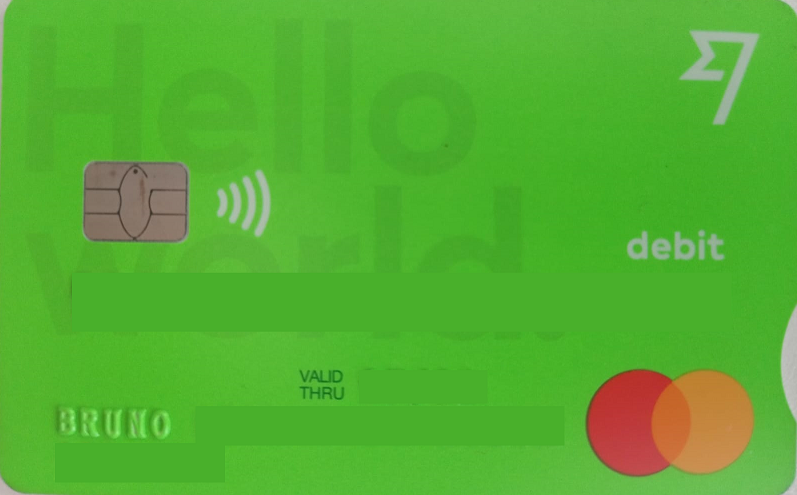
\includegraphics[width=6cm]{Bilder/eigenes_Bild_Karte.png}}
   \caption{Eine Smartcard und deren eingebetete Mikrochip\\(eigene Quelle)}
   \label{fig:eigenes_Bild}
\end{figure}
\vfill

Sie wurde vor mehr als 40 Jahren erfunden und ihr Ziel ist die Sicherheit von Kartenzahlung und allgemeine
Authentifizierungsverfahren zu erhöhen \cite{refip:JFSB}. Sie unterscheiden sich von traditionelen 
Magnetstreifenkarten, weil sie verschiedene Authentifizierungsmethoden ermöglichen auch ohne eine direkte 
Verbindung zur Bank \cite{refbook:ATMS}. Im folgenden wird der Authentifizierungsprozess einer Smartcard 
\ref{fig:refbook_ATMS} dargestellt. 

\vfill
%htb
\begin{figure}[H]
    \centering{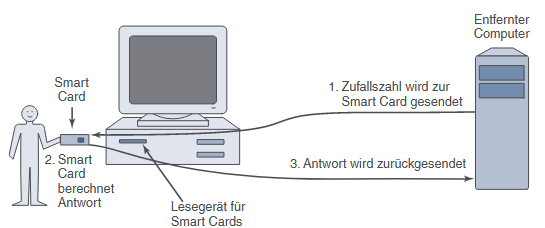
\includegraphics[width=10cm]{Bilder/refbook_ATMS.png}}
   \caption{Authentifizierungsprozess von Smartcards\\(Tanenbaum, 2009, S.755)}
   \label{fig:refbook_ATMS}
\end{figure}
\vfill

Die meisten Angriffe bei Smartcards geschehen laut \cite{refmas:ASSS} auf Hardwareebene.
Er beschreibt folgende Techniken für Angriffe:

\begin{itemize}
    \item Protokollanalyse: schwache Konzipierung oder mangelnde Verschlüsselung ermöglichen Zugang 
    zum Klartext; 
    \item Relay: Konzentriert auf kontaktlose Smartcards, um den Inhalt umzuleiten;
    \item Seitenkanal-Attacken: zielt nicht direkt den Inhalt der Kommunikation, sondern versucht sie
    zu stören;
    \item Hardware Reverse Engineering: Verständnis über die Algorithmen oder Extrahieren des Schlüssels.
\end{itemize}


Die Schutzmaßnahmen können laut \cite{refmas:ASSS} in drei Gruppen aufgeteilt werden: physikalisch,
logisch und organisatorisch. Auf der physikalischen Ebene soll die Hardware robust aufgebaut werden,
um Angriffe schwieriger zu gestalten. Diese Konstruktion soll komplexer, also mit zusätzlichen Elementen erstellt
werden. 

\textbf{Ich würde vorschlagen, dass wir besser erläutern, was robust hier heißt. Und wir sollen vllt
aucht die anderen Ebenen, logisch und organisatorisch erläutern.}


Letztendlich sollen Smartcards in der Lage sein, Angriffe schnell zu detektieren und zu verhindern.
Zu dieser Ebene gehört auch das Sperren der Karte, falls die Karte unautorisiert genutzt wurde, 
die Überprüfung von Logdateien, um Klone zu identifizieren und die Verwendung von Zwei-Faktor-
Authentisierung.


Angriffe Smartcards
Smartcards sind auf Hardwareebene extrem sicher. Sie werden von https://www.emsec.ruhr-uni-bochum.de/media/attachments/files/2012/04/Master-Arbeit-public.pdf
auch als in Hardware gegossener Tresor für Informationen bezeichnet. Wenn eine Smartcard für das Bezahlen verwendet wird,
ist kein Backend-System nötig, denn alle wichtigen Informationen wie das Guthaben sind direkt auf der Karte gespeichert. Aus diesem Grund 
können keine Daten abgefangen werden, die auf dem Weg vom Lesegerät zum Backend-System sind, was den Bezahlprozess deutlich sicherer macht.
Zudem muss jede Kommunikation vom Lesegerät initiiert werden, die Karte selber startet also nie eine Kommunikation. Da die wichtigsten Daten
direkt auf der Karte gespeichert sind, muss ein Angriff auf die Hardware gestartet werden, um an relevante Informationen zu kommen.
Eine andere Möglichkeit wäre es die Schwachstellen eines bestimmten Protokolls das für die Kommunikation verwendet wird auszunutzen.

Gegenmaßnahmen:
Um einen Angriff auf die Hardware möglichst zu vermeiden, ist es sinnvoll den Chip nicht rekonstruierbar zu machen,
das heißt es werden keine Standardzellen oder ähnliches verwendet.
Zusätzlich spielt die Verschlüsselung der Daten eine große und erhöht die Sicherheit enorm.
Außerdem können Mechanismen in die Smartcard eingebaut werden, die zum Beispiel permanent die Spannung oder Frequenz
überprüfen und sobald etwas nicht dem Normalzustand entspricht, wird der Chip ausgeschaltet, sodass kein Lesegerät mit der 
Karte kommunizieren kann. Letztlich ist es wichtig, dass jede Karte individuell ist, sodass ein erfolgreicher Angriff kein 
Sicherheitsrisiko für andere Karten dargestellt. Dazu wären asymmetrische Verschlüsselungsverfahren sinnvoller als 
symmetrische, da jede Karte bei asymmetrischer Verschlüsselung einen öffentlichen und privaten Schlüssel hat und nicht jeder den selben 
Schlüssel haben.




- Smartcards sind auf der Hardwareebene extrem sicher. https://www.emsec.ruhr-uni-bochum.de/media/attachments/files/2012/04/Master-Arbeit-public.pdf bezeichent Smartcards auch als 
  ein in Hrdware gegossener Tresor für Informationen. 
- das Guthaben oder der Verfügungsrahmen wird direkt auf der Karte gespeichert, sodass der ganze Prozess nicht über ein Backend-System laufen muss
- die Komunikation wird immer vom Leser initiiert, die Karte reagiert nur
- Angriffe richten sich direkt gegen die Hardware, nicht etwa Socail Engineering 
- Analyse von übertragenen Daten --> Rückschlüsse auf Schwachstellen vom verwendeten Protokoll

Gegenmaßnahmen:
- damit der Chip nicht rekonstruierbar ist, sollte dieser möglichst Komplex sein, keine Standardzellen oder ähnliches einbauen
- Zusätzlich lassen sich die Inhalte von Bussen und Speichern bereits auf Hardwareebene
  durch Scrambling, das heißt das Vertauschen von Adressen, oder durch Verschlüsselung
  der Daten schützen [2, S.540f][2, S.544f]. Schutzschichten, die den gesamten Chip umgeben
  und von diesem permanent auf ihre Unversehrtheit geprüft werden, bilden eine weitere
  Barriere die interne Funktionsweise zu analysieren [2, S.539f]. Andere Sensoren, etwa
  zur Überwachung von Spannung oder Frequenz, können den Chip abschalten, sobald
  diese einen Betrieb außerhalb der zulässigen Spezifikationen und damit einen möglichen
  Angriff erkennen
- Seitenkanal Angriffe können zum Beispiel durch immer gleich bleibenden Stromverbrauch verhindert werden
- Grundvoraussetzung für ein sicheres System ist eine Authentifizierung der jeweiligen
  Gegenstelle bei der Kommunikation, da nur so sicher gestellt werden kann, dass es sich
  beim Kommunikationspartner nicht um einen Angreifer handelt [2, S.571]. Obwohl es
  auch möglich ist, allein die Integrität übertragener Daten zu schützen, werden diese
  oftmals zusätzlich verschlüsselt, sodass auch die Vertraulichkeit gewährleistet ist [2, S.570].
  Alle für derartige kryptografische Operationen eingesetzten Algorithmen sollten öffentlich
  bekannt und untersucht sein, um Sicherheitslücken soweit wie möglich auszuschließen [30,
  S.9].
  Bei der Implementierung der Algorithmen ist darauf zu achten, dass ein konstantes
  Zeitverhalten gewährleistet wird, das heißt unabhängig von den Eingabedaten die gleiche
  Ausführungszeit benötigt wird, um so darauf basierende Seitenkanalattacken zu unterbin-
  den [2, S.560f]. Zufallszahlen, die unter anderem bei der Authentifizierung eine wichtige
  Rolle spielen, sind auf kryptografisch sichere Weise zu erzeugen
- Auf organisatorischer Ebene ist es wichtig, die Verwendung von kartenindividuellem
  Schlüsselmaterial sicherzustellen, um zu verhindern, dass ein erfolgreicher Angriff auf
  eine Karte auch andere Karten unmittelbar gefährdet. Dies geschieht entweder durch den
  Einsatz asymmetrischer Kryptografie, bei der für jede Karte eigenes Schlüsselmaterial
  generiert und von einer zentralen Instanz signiert wird, oder durch die so genannte
  Key Diversification bei Verwendung symmetrischer Kryptografie. Hierbei wird unter
  Einsatz einer Einwegfunktion ein kartenindividueller Schlüssel von einem Hauptschlüssel
  abgeleitet und nur der abgeleitete Schlüssel auf der Karte gespeichert [30, S.22].
  Sollte es zu einem Verlust oder einem erfolgreichen Angriff auf eine Karte kommen,
  muss es möglich sein, diese Karte (genauer: ihr Schlüsselmaterial) im System zu sperren,
  indem entsprechende Sperrlisten gepflegt werden [2, S.572]. Dass eine Karte angegriffen
  und beispielsweise geklont wurde, lässt sich durch das Erstellen von Logeinträgen für
  jede Verwendung und deren Überprüfung auf Unregelmäßigkeiten erkennen

\subsection{Fazit}


\textbf{Herr Rutter hat vorgeschlagen, dass wir unsere Meinung zu den beiden Elementen geben und uns für 
eins entscheiden. Wir müssen unsere Entscheidung begründen. Damit kriegen wir eine sehr gute Note sagte er.}